\vspace{-0.2cm}
\section{Introduction}
\vspace{-0.2cm}

Large language models (LLMs) are a useful tool for reasoning in scientific domains such as math and coding~\citep{shao2024deepseekmath,lozhkov2024starcoder,team2024codegemma}. An aspirational property of LLMs in such settings is their ability to implement \emph{meta-strategies} or \emph{algorithms} that use test-time computation to generate improved responses. However, modern LLMs do not implement such strategies reliably. For instance, consider a problem that requires models to detect and revise (or ``self-correct'') their own responses in order to eventually arrive at the best possible final response. This self-correction capability has been shown to be severely lacking in current LLMs, especially in the absence of external input (also called \emph{intrinsic self-correction})~\citep{huang2023large, kamoi2024can}. 

\begin{figure}[!ht]
    \centering
    \begin{subfigure}{0.48\linewidth}
        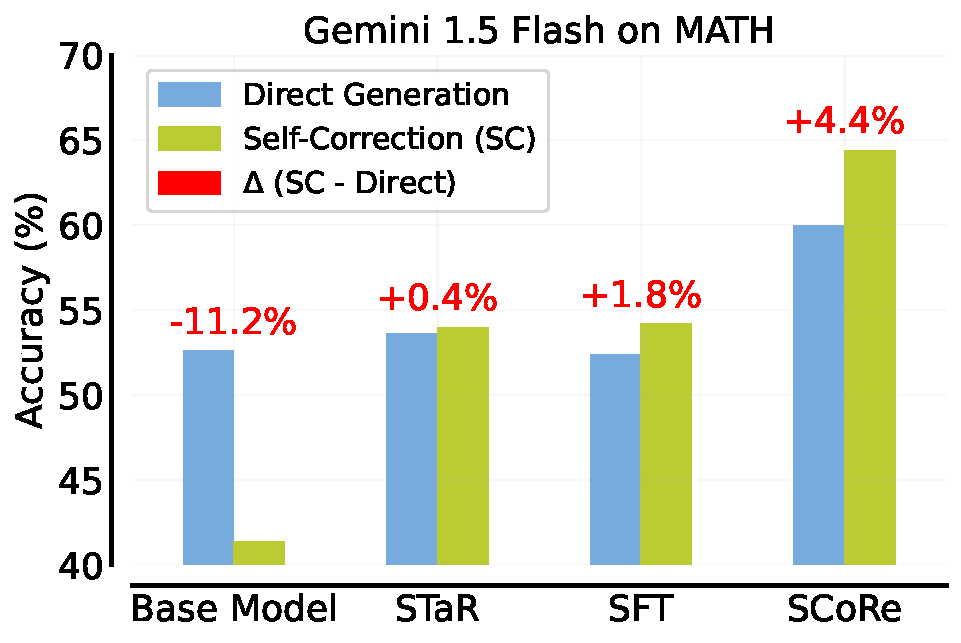
\includegraphics[width=\linewidth]{assets/main_math_bar.pdf}
        \label{sub:main_math}
    \end{subfigure}
    ~
    \begin{subfigure}{0.48\linewidth}
        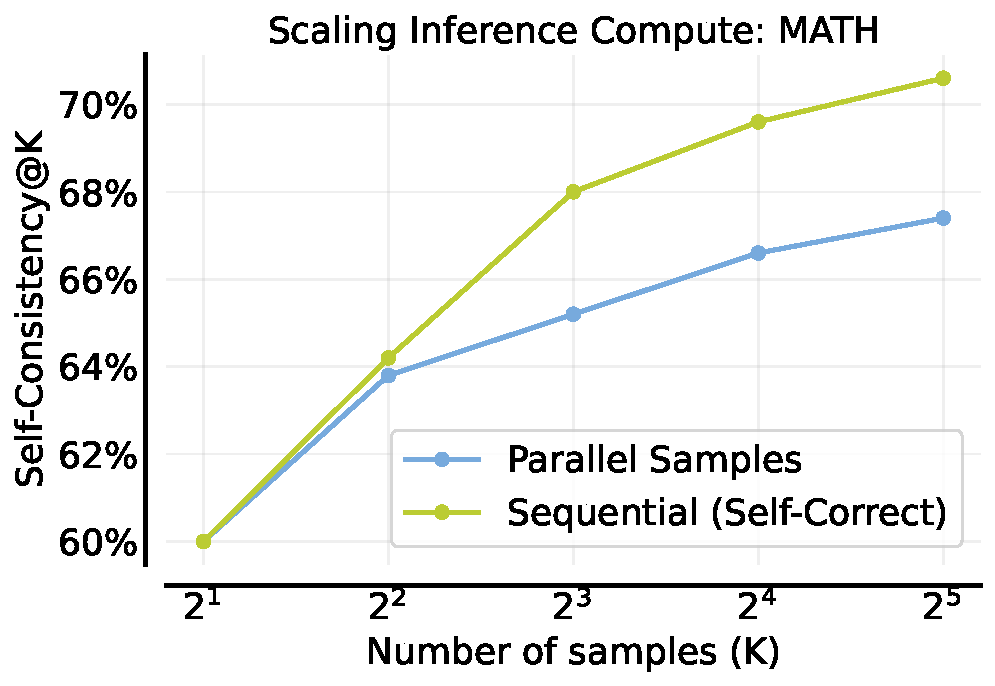
\includegraphics[width=\linewidth]{assets/inference_compute_scaling.pdf}
        \label{sub:inference_math}
    \end{subfigure}
    \vspace{-0.55cm}
    \caption{\footnotesize{\textbf{Left:} \methodname{} achieves state-of-the-art self-correction performance on MATH; \textbf{Right:} \methodname{} inference-time scaling: spending samples on \emph{sequential} self-correction becomes more effective than only on \emph{parallel} direct samples~(Section~\ref{sec:inference}).}}
    \label{fig:main}
    \vspace{-0.35cm}
\end{figure}

To make progress towards teaching LLMs to implement meta-strategies for challenging inputs, we study a special instance of training LLMs to perform self-correction to fix their mistakes ``on-the-fly''. This should be possible: on many queries where current LLMs fail, they possess the underlying ``knowledge'' needed to arrive at the correct response but are unable to correctly elicit and draw inferences about their own knowledge when needed~\citep{yang2024large}. For example, strong LLMs can often successfully complete a sub-part of a math proof when prompted with the remainder, but may not be able to complete it from scratch. In a similar vein, leveraging their previous responses should, in principle, enable LLMs to improve their subsequent ones. Despite this, self-correction has remained elusive, highlighting the need to go beyond existing training paradigms.

\textbf{How can we imbue LLMs with self-correction abilities?} Prior attempts for self-correcting LLMs either rely on prompt-engineering~\citep{madaan2023self, kim2023language} or on fine-tuning models specifically for self-correction. While the former approaches often fail to perform meaningful intrinsic self-correction, fine-tuning approaches require running multiple models during inference, such as a separate refinement model~\citep{havrilla2024glore,welleck2023generating}, or rely on ``teacher'' supervision to guide the process of self-correction~\citep{qu2024recursive}. With the use of separate models of teacher supervision, self-correction does not necessarily outperform parallel, independent attempts. We develop an approach that is effective at self-correction \emph{without} these requirements. Our approach, \textbf{S}elf-\textbf{Co}rrection via \textbf{Re}inforcement Learning (\methodname{}), trains only a single model that can both produce a response to a problem and \emph{also} correct errors without any oracle feedback.

To develop \methodname{}, we start by analyzing the shortcomings of SFT-based approaches (e.g., STaR~\citep{zelikman2022star}) and na\"ive RL that optimizes final response correctness for teaching self-correction. We find that such approaches fall prey to either:  \textbf{(1)} \emph{distribution shift}, where the trained model is able to correct errors made by the base model that generated the data, but these gains do not transfer to self-correction under the learned model's own mistakes; or \textbf{(2)} \emph{behavior collapse}, where the learning progress simply learns to produce the best first-attempt response followed by superficial or no modifications in the second attempt. To address these issues, \methodname{} trains for self-correction directly via on-policy, multi-turn RL. To prevent behavior collapse, \methodname{} employs two-stage training: in the first stage, it produces an initialization that is less susceptible to behavior collapse  by training to correct second-attempt responses while constraining the first-turn distribution to be close to the base model; followed by training on both attempts to maximize reward in the second stage. Crucially, the second stage of multi-turn RL employs a reward shaping term that rewards ``progress'' towards self-correction as opposed to the correctness of the final response.  






Our main contribution is \methodname{}, a multi-turn RL approach for teaching LLMs how to correct their own mistakes. To the best of our knowledge, \methodname{} is the first approach to attain significantly positive intrinsic self-correction: relative to base Gemini models, our method attains an absolute \textbf{15.6\%} gain on self-correction for reasoning problems from MATH~\citep{hendrycksmath2021} and an absolute \textbf{9.1\%} gain on coding problems from HumanEval~\citep{chen2021evaluating}. We additionally motivate the design of \methodname{} by extensively studying the failure modes of SFT and standard RL approaches, which broadly indicate that reinforcement learning plays an essential role in \emph{self-trained} self-correction.
